\chapter{Anhang}

\begin{figure}[!ht]
    \centering
    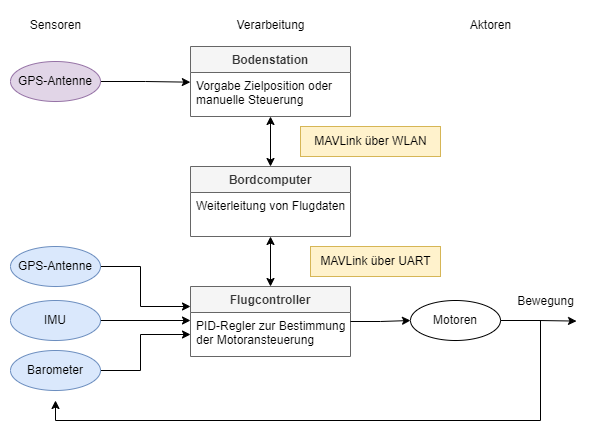
\includegraphics[width=\linewidth]{images/001_vereinfacht-Page-3_default.drawio.png}
    % oder mehrere Bilder, dann aber IMMER MIT \hfill !!!!
    %\subfloat[Bild 1]{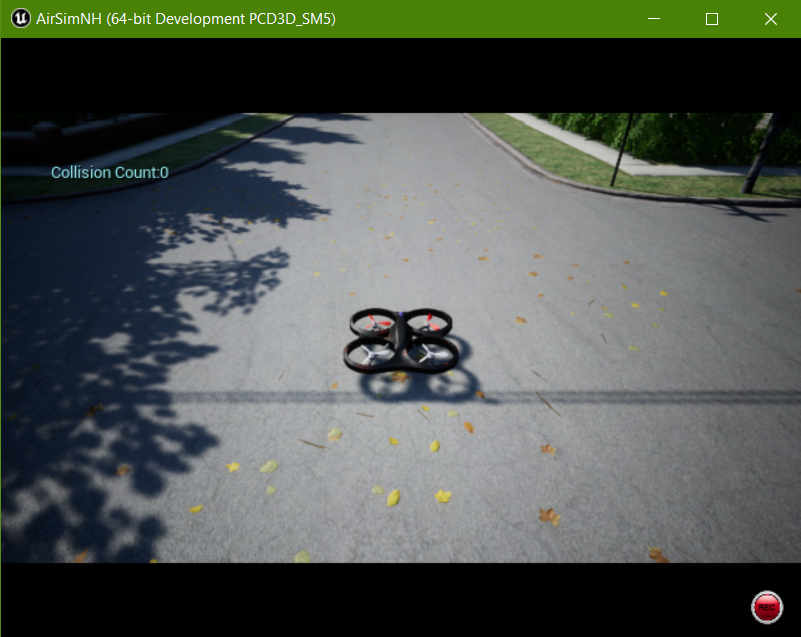
\includegraphics[width=0.4\textwidth]{images/sim_initial.png}}\hfill
    %\subfloat[Bild 2]{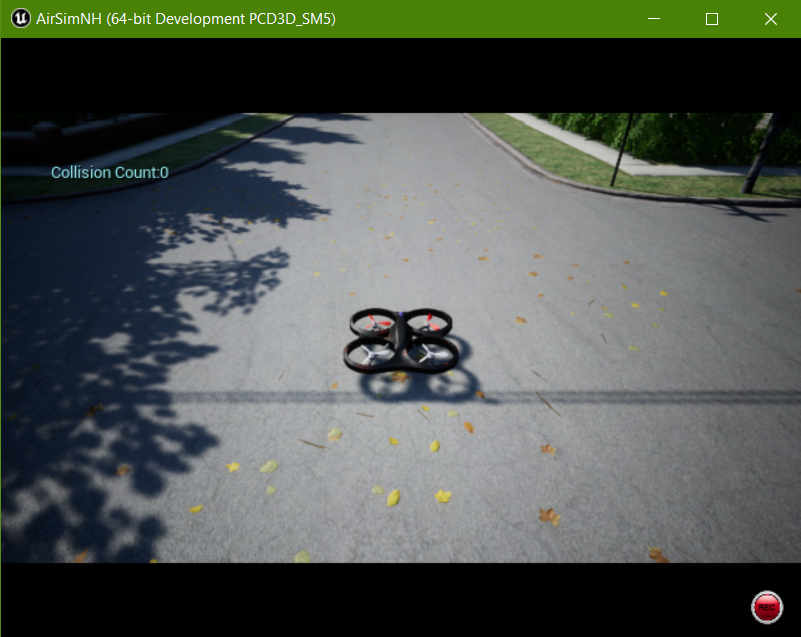
\includegraphics[width=0.4\textwidth]{images/sim_initial.png}}\hfill
    \caption[Beschreibung des Systems Drohne-Bodenstation]{Beschreibung des Systems Drohne-Bodenstation: Grau hinterlegt die Bestandteile aus Tabelle \ref{tab:system_intro}; Gelb hinterlegt das jeweilige Kommunikationsprotokoll; Blau hinterlegt vorhandene Sensoren; Lila hinterlegt optionale Sensoren}
    \label{fig:system_intro}
\end{figure}

\begin{figure}[!ht]
    \centering
    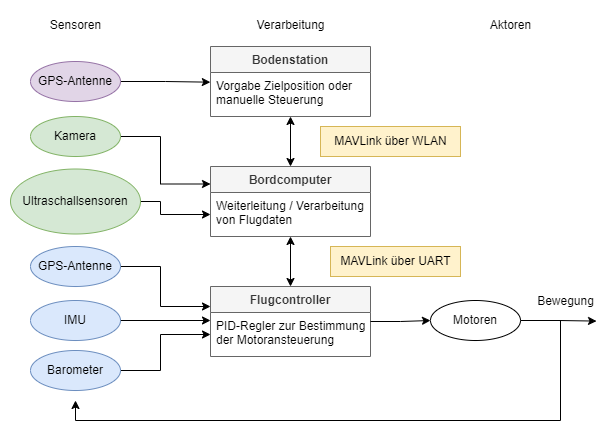
\includegraphics[width=\linewidth]{images/001_vereinfacht-Page-3_erweitert.drawio.png}
    \caption[Beschreibung des erweiterten Systems Drohne-Bodenstation]{Beschreibung des erweiterten Systems Drohne-Bodenstation: Grün hinterlegt neu vorgesehene Sensoren}
    \label{fig:system_added_sensors}
\end{figure}

\begin{figure}[!ht]
    \centering
    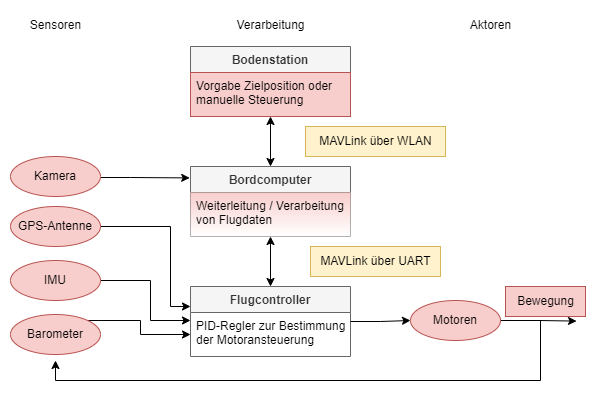
\includegraphics[width=\linewidth]{images/001_vereinfacht-Page-3_simuliert.drawio.png}
    \caption[Beschreibung des Systems zur Simulation HIL]{Beschreibung des Systems zur Simulation HIL: Hell-rot dargestellt die von der Simulation übernommenen Aufgaben}
    \label{fig:system_sim}
\end{figure}

\begin{figure}[!ht]
    \centering
    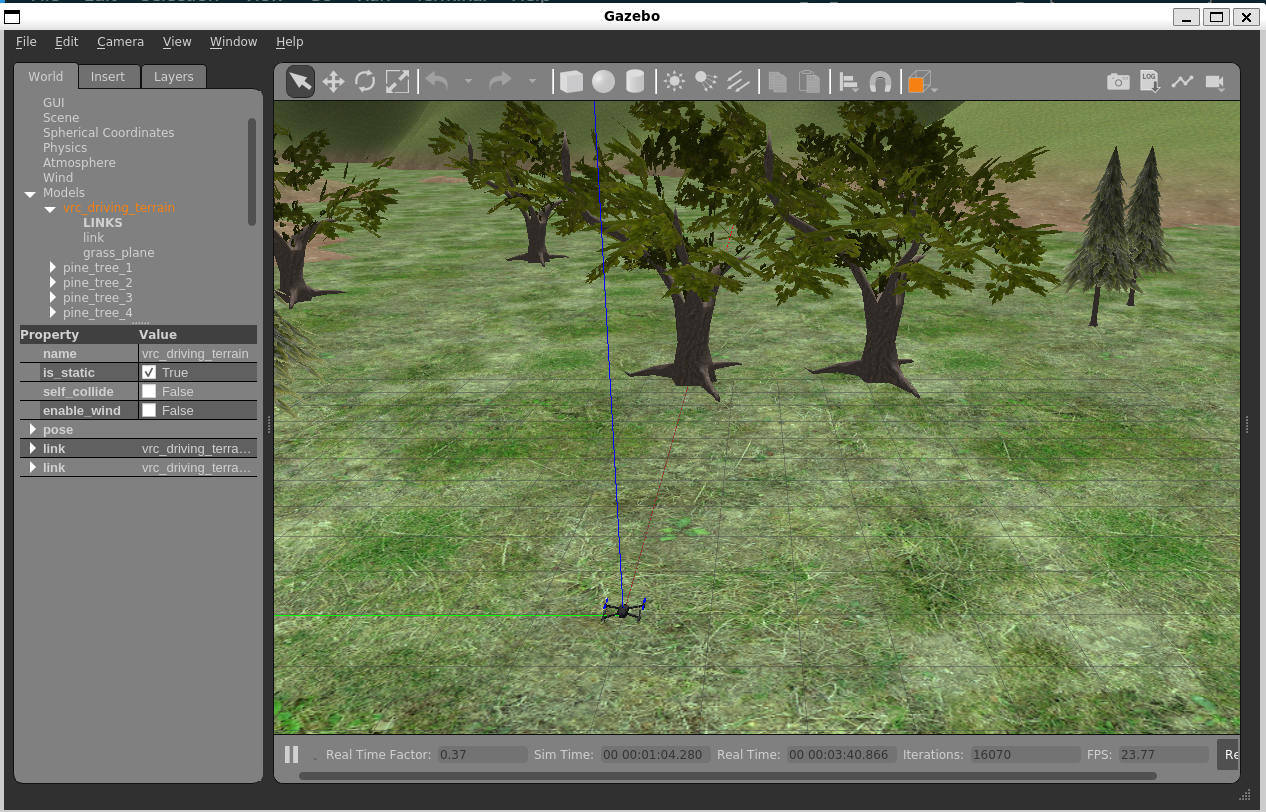
\includegraphics[width=\linewidth]{images/sim_gazebo.png}
    \caption[Ansicht Gazebo Simulator]{Erste Ansicht von Gazebo bei der Simulation von Avoidance: Relativ klein im Vordergrund die simulierte Drohne mit Koordinatenachsen (Rot, Grün, Blau), im Hintergrund die Welt mit Bäumen, auf linker Seite ein Konfigurationsmenü von Gazebo}
    \label{fig:sim_gazebo}
\end{figure}

\begin{figure}[!ht]
    \centering
    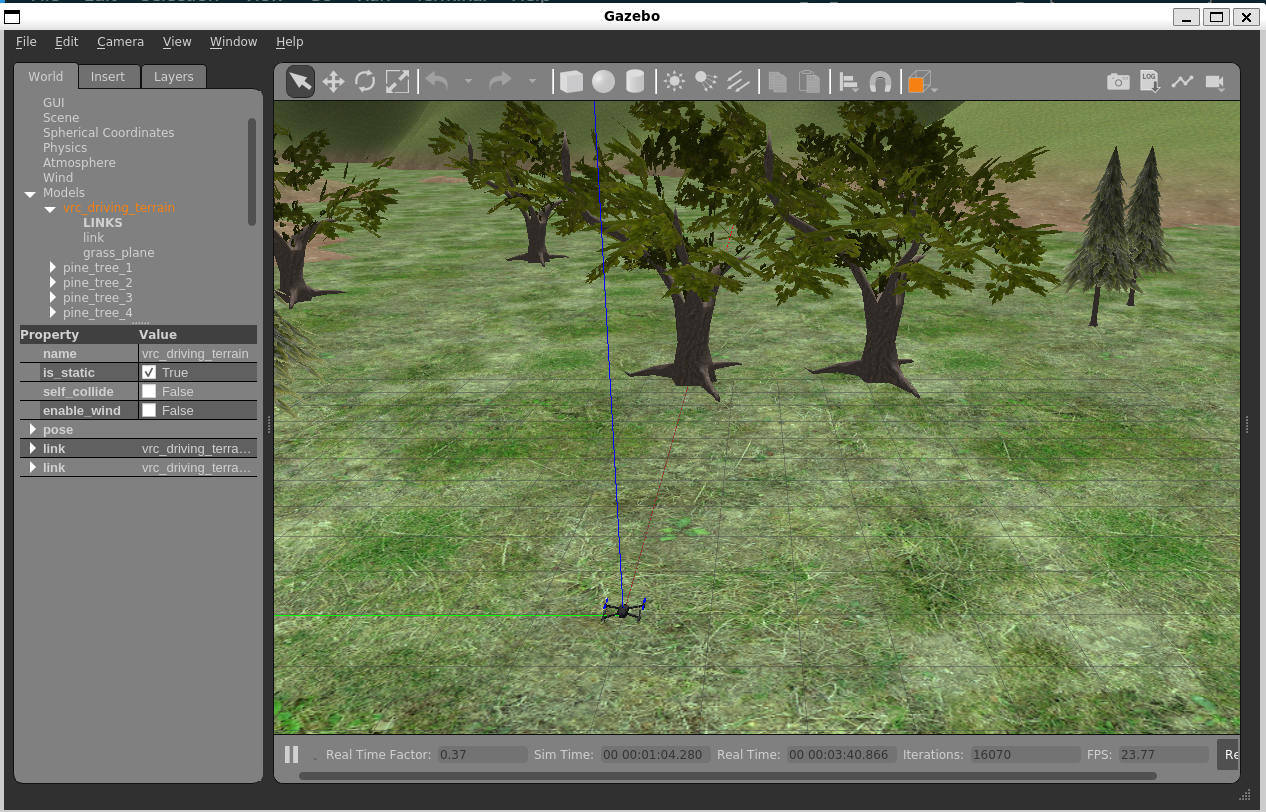
\includegraphics[width=\linewidth]{images/sim_gazebo.png}
    \caption[Ansicht Gazebo Simulator]{Erste Ansicht von AirSim bei der Blocks-Simulation: im Vordergrund die simulierte Drohne, im Hintergrund ein großer Quader und eine Kugel}
    \label{fig:sim_airsim}
\end{figure}

\begin{figure}[!ht]
    \centering
    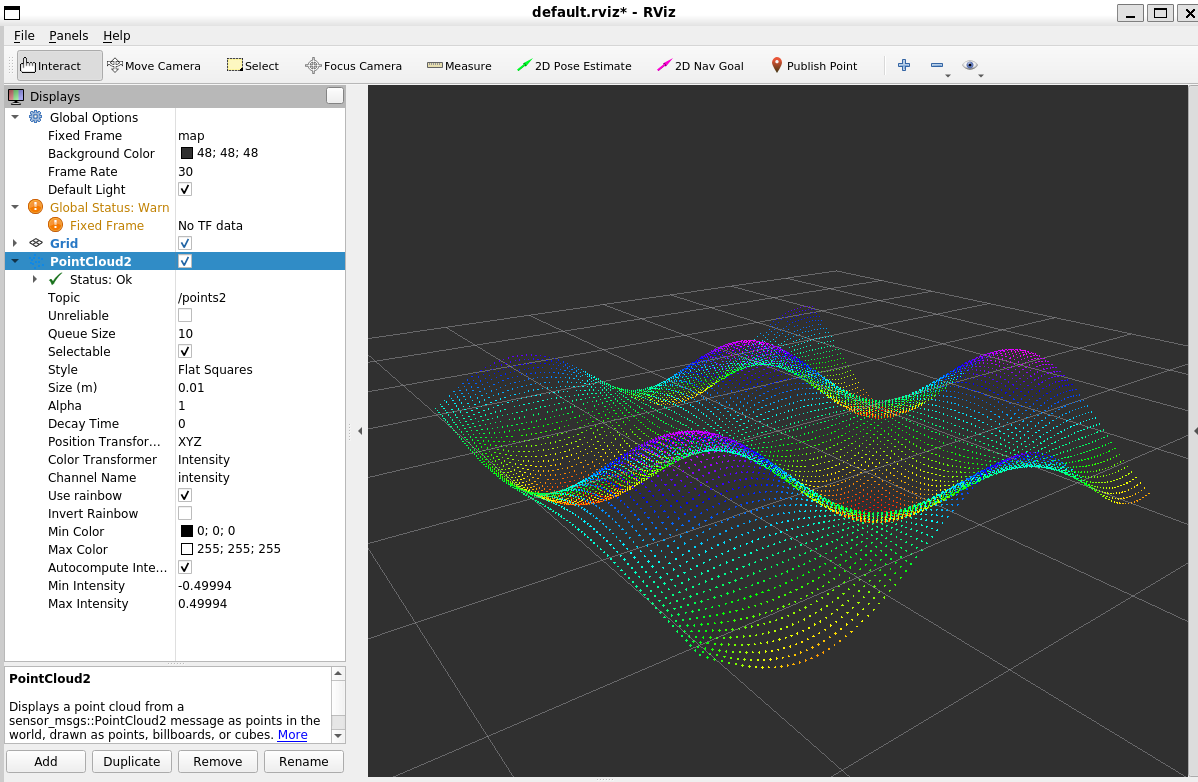
\includegraphics[width=\linewidth]{images/ultra_pc_example.png}
    \caption{Vorgefertigtes Beispiel zur Punktwolke}
    \label{fig:ultra_pc_ex}
\end{figure}

\begin{listing}[!ht]
    \pycode{snippets/pcl_test.py}
    \caption{Eigener Beispielcode zur Veröffentlichung von 5 Punkten um Koordinatenursprung}
    \label{listing:pcl_test.py}
\end{listing}

\begin{listing}[!ht]
    \shcode{snippets/setup_gazebo.sh}
    \caption{Setup-Script für Gazebo Simulation}
    \label{listing:setup_gazebo.sh}
\end{listing}

\begin{listing}[!ht]
    \shcode{snippets/setup_stereopi.sh}
    \caption{Setup-Script auf Stereopi}
    \label{listing:setup_stereopi.sh}
\end{listing}
